\documentclass{article}

% if you need to pass options to natbib, use, e.g.:
% ©PassOptionsToPackage{numbers, compress}{natbib}
% before loading nips_2016
%
% to avoid loading the natbib package, add option nonatbib:
% \usepackage[nonatbib]{nips_2016}

\usepackage[final]{nips_2016}

% to compile a camera-ready version, add the [final] option, e.g.:
% \usepackage[final]{nips_2016}

\usepackage[utf8]{inputenc} % allow utf-8 input
\usepackage[T1]{fontenc}    % use 8-bit T1 fonts
\usepackage{hyperref}       % hyperlinks
\usepackage{url}            % simple URL typesetting
\usepackage{booktabs}       % professional-quality tables
\usepackage{amsfonts}       % blackboard math symbols
\usepackage{amssymb}
\usepackage{amsmath}
\usepackage{bbm}
\usepackage{nicefrac}       % compact symbols for 1/2, etc.
\usepackage{microtype}      % microtypography
\usepackage{caption}
\usepackage{float}
\usepackage{graphicx}
\usepackage{wrapfig}
\usepackage{authblk}
\usepackage{subcaption}

\graphicspath{ {./} }

\title{A multi-modal neural network for learning cis and trans regulation of stress response in S. cerevisiae}

% The \author macro works with any number of authors. There are two
% commands used to separate the names and addresses of multiple
% authors: \And and \AND.
%
% Using \And between authors leaves it to LaTeX to determine where to
% break the lines. Using \AND forces a line break at that point. So,
% if LaTeX puts 3 of 4 authors names on the first line, and the last
% on the second line, try using \AND instead of \And before the third
% author name.

\author[1,2,3]{Boxiang Liu}
\author[4]{Nadine Hussami}
\author[3,5]{Avanti Shrikumar}
\author[3]{Tyler Shimko}
\author[6]{Salil Bhate}
\author[6]{Scott Longwell}
\author[2,3]{Stephen Montgomery}
\author[3,6]{Anshul Kundaje}
\affil[ ]{$^1$Departments of Biology, $^2$Pathology, $^3$Genetics, $^4$Statistics, $^5$Computer Science, and $^6$Bioengineering, Stanford University}
\affil[ ]{\textit{\{bliu2,nadinehu,avanti,tshimko,bhate,longwell,smontgom,akundaje\}@stanford.edu}}

\begin{document}

\maketitle

\begin{abstract}

Understanding gene regulatory mechanisms is a central problem in computational biology. Here, we explore the use of interpretable multi-modal neural networks to learn cis and trans regulation of stress response in the budding yeast \textit{Saccharomyces cerevisiae}. We formulate the problem as a regression task, where the goal is learn a model that can accurately predict the real-valued gene expression of all genes across 173 different stress conditions based on two complementary regulatory inputs - a cis component represented by the raw promoter sequence of each gene and a trans component represented by the real-valued expression of a subset of regulatory genes (transcription factors and signaling molecules). The multimodal neural network includes a convolutional module to learn predictive patterns from the raw promoter sequences, a dense module to derive features from regulator expression and an integration module that learns cis-trans interactions. We use a variety of cross-validation settings to evaluate the performance of the model (held-out genes, held-out stress conditions). In all cases, the models achieve high performance and substantially outperform other state-of-the-art methods such as boosting algorithms that pre-defined cis-regulatory features (known motifs). We then use an efficient backpropagation algorithm that we recently developed to interpret the model. We interpret the model to reveal dynamic promoter sequence motif grammars, trans regulator modules and motif-regulator associations affecting individual genes and gene modules in diverse stress conditions. Our model correctly identifies known master regulators such as MSN4/MSN2, USV1, YVH1 as well as several stress-specific factors. We also use our models to perform in silico knock-out/knock-in experiments. In a MSN2/4 knockout experiment, we demonstrate that in silico predictions of target gene changes strongly correlate with the results of the corresponding knockout microarray experiment.
  
\end{abstract}

\section{Introduction}

The accurate prediction of gene expression based on the interaction between transcription regulators and DNA sequence is a critical milestone toward fully comprehending cellular regulome. Several studies have contructed computational models to tackle this problem. Some use the sequence information \cite{Bussemaker:2001ft,Phuong:2004kk}, while others use the transcription regulator expression \cite{Soinov:2003iz,Segal:2003ks}. In particular, GeneClass\cite{Middendorf:2004gta} and BDTree\cite{Ruan:2006hl} model gene expression based on the interaction between sequence motif and regulator, and thus can discover previously unknown regulatory patterns. However, due to modeling assumptions, both methods require discretized expression values, which severely limits their utility. Further, they both assume prior knowledge on sequence motifs, which is unavailable in certain cases. Perhaps unsurprisingly, aforementioned studies all use yeast as the model organism. The budding yeast \textit{Saccharomyces cerevisiae} possesses a relatively simple transcriptional regulatory architecture governed primarily by promoter sequence directly upstream of the gene. Such architecture has very few long range interactions such as those in higher-order organisms, and is ideal for computational modeling. 


We present a deep neural network architecture to address the limitations with previous methods. Our architecture models gene expression as the interaction between trans (signaling molecules and transcription factors) and cis (1kbp promoter sequence) regulatory components. Our model automatically extract sequence motifs from raw sequences, thus eliminating the need for prior knowledge and feature engineering. Our model predicts gene expression values in $\mathbb{R}$, akin to microarray and sequencing measurement. We demonstrate that our model outperforms the state-of-the-art methods, and provides sensible prediction concordant with existing knowledge of yeast biology.


\section{Methodology}

\subsection{Sequence module}
We treat one-hot encoded promoter sequences as black-and-white images of size $\{0,1\}^{4 \times 1000}$. The promoter sequences contain information about transcription factor binding motifs, each representing a consensus sequence (e.g. 'TGATCA'). Like an object in natural images, a motif appears in multiple promoter sequences and a given promoter can contain several instances of the same motif with slight variations. We use a 2-layer convolutional neural networks to detect such motifs. Mathematically, the 2D convolution layers with ReLU activation can be written as: 

\begin{equation} \label{eq1}
x_{ij}=\max \{ 0, \sum_{a=1}^{4} \sum_{b=1}^{l} W_{abj}^{seq} s_{(a)(i+b)} + b^{seq}\}
\end{equation} 

Where $s$ represents sequence input, $W^{seq}$ represents the weight for convolutional filters, $i$ represents the genomic location, $j$ represents filter number, $b^{seq}$ represents the bias, and $l$ represents the filter length. We use $l=9$ and $J=50$ filters for both convolutional layers with a subsampling rate of 1. To keep model prediction invariant to small motif shifts along the genomic axis, we apply 1D maxpooling with a subsampling rate of 4 after each convolutional layer. We applied batch normalization before each ReLU activation to mitigate covariate shifts during training and to accelerate learning. Since both strands of DNA encode identical information, we incorporated the reverse complement sequences into our model, effectively doubling the number of training examples, and used filter pairs with mirroring weights to detect each motif \cite{Anonymous:_KTX_iBy}. We used a fully connected layer with 512 units to integrate information across filters. 


\subsection{Regulator module}
Transcription factors and signaling molecules interact with each other through bi-, tri-molecular and even higher order reactions with no genomic-spatial constraint. We model the regulator input with a fully connected layer of 512 hidden units. Mathematically, 

\begin{equation} \label{eq2}
y=\max \{0, W^{reg}r + b^{reg}\}
\end{equation}

\subsection{Integration module}
In principle, the output from sequence module represents gene-specific information, and that from the regulator module represents condition-specific information. Treated separately, neither module will be able to predict the gene-condition interactions critical for accurate final prediction. We integrate two separate sources of information through a simple concatenation layer, and use a 2-layer fully connected network to model the interaction between motifs and regulators. 

\subsection{Dataset and Pre-processing}

We utilized the Gasch \cite{Gasch:2000wl} dataset which used microarray to measure a total of 6100 genes under 173 experimental conditions. The measurements were given as $log_2$ expression values representing the fold change w.r.t. the untreated reference condition. We used 1kbp sequences upstream of the transcription start site as the sequence predictors and a set of 472 transcription factors and signaling molecules as the regulator predictors. We used a 80-10-10 split among training, validation, and test datasets.


% \subsection{Training methodology}
% We trained our models using SGD with a learning rate of 0.01 and momentum of 0.5. We decrease the learning rates by half every five epoch if no improvement in validation accuracy is observed. All training were performed on Nvidia GeForce GTX 970 using Keras 1.2.2 with Tensorflow backend.


\section{Results}

\subsection{Regression and Classification Performances}
We compared our model against two state-of-the-art models, GeneClass \cite{Middendorf:2004gta} and BDTree \cite{Ruan:2006hl}, using the same dataset by Gasch et al \cite{Gasch:2000wl}. The GeneClass model is a boosted alternating decision tree, and the BDTree model is a bidirectional regression tree. We trained our model to predict real-valued expression levels as well as discrete labels in $\{-1,0,1\}$ to represent upregulation, baseline, and downregulation. In the classification task, the dataset is discretized such that expression values in $[-\infty,-0.5]$ are converted to -1, $[-0.5,0.5]$ to 0, and $[0.5,\infty]$ to +1. Our best model outperformed the previous state-of-the-art by 16.6\% (Table \ref{table:classification performance}). In addition, our model achieved a pearson correlation of 0.82 for the regression task on the test set (Figure \ref{fig:correlation}). For regression, we could not compare our models because GeneClass or BDTree only reported classification results.

\begin{table}[!hbt]
\caption{Classification performance}
\centering
 \begin{tabular}{|c | c|} 
 \hline
 Method & Accuracy \\
 \hline
 GeneClass & 60.9\% \\ 
 \hline
 BDTree & 62.9\% \\
 \hline
 DNN & \textbf{79.5\%} \\
 \hline
\end{tabular}
\quad
\centering
 \begin{tabular}{|c | c c c|} 
 \hline
 {} & \multicolumn{3}{|l|}{Predicted by DNN} \\
  & Down & Baseline & Up \\ 
 \hline
 Down & 10.14 & 7.47 & 0.13 \\
 \hline
 Baseline & 3.29 & 59.77 & 3.02 \\
 \hline
 Up & 0.18 & 6.42 & 9.59 \\
 \hline
\end{tabular}
\label{table:classification performance}
\end{table}

\subsection{Recovering Known Motifs}
Unlike GeneClass and BDTree which rely on existing motif annotations, our model learn filter weights and extracts motif information automatically.  We found that our model learns both known and \textit{de novo} motifs. Figure 1 shows four known motifs recovered by our model. 


\begin{figure}[h]
    \centering
    \begin{subfigure}{.475\textwidth}
        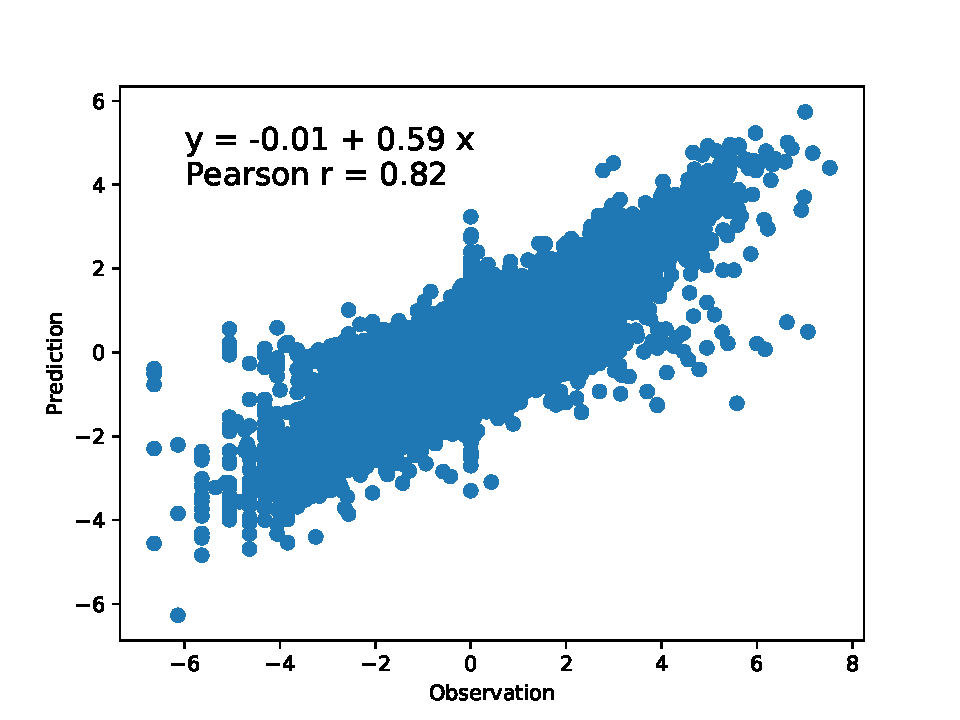
\includegraphics[width=\textwidth]{fig/correlation_tensor_product.pdf}
        \caption[Correlation]{Correlation}
    \end{subfigure}\hfill
    \parbox{.475\textwidth}{
        \begin{subfigure}{.475\linewidth}
            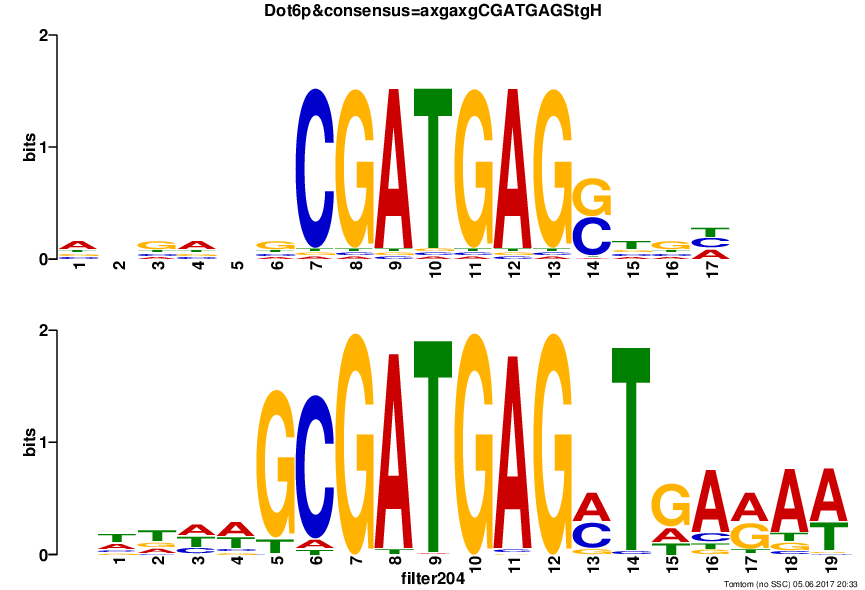
\includegraphics[width=\textwidth]{fig/tomtom/dot6p_2.png}
            \caption{DOT6P}
    \end{subfigure}
    \begin{subfigure}{.475\linewidth}
            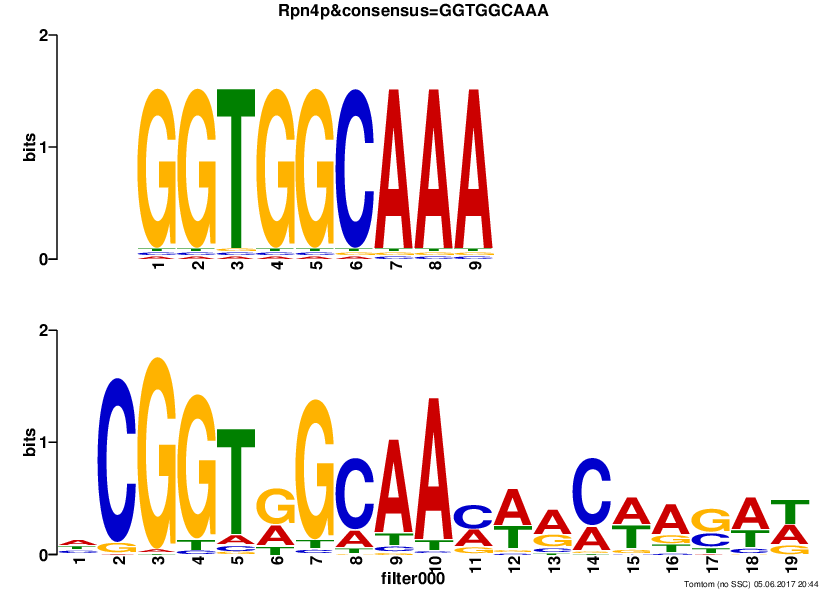
\includegraphics[width=\textwidth]{fig/tomtom/rpn4p.png}
            \caption{RPN4P}
    \end{subfigure}\\
    \begin{subfigure}{.475\linewidth}
            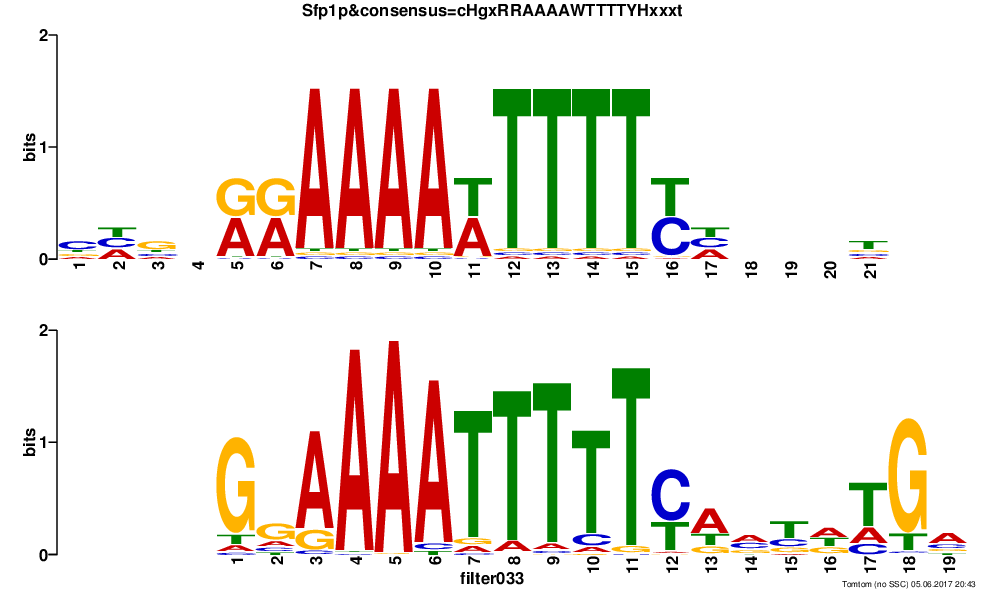
\includegraphics[width=\textwidth]{fig/tomtom/sfp1p_2.png}
            \caption{SFP1P}
    \end{subfigure}
    \begin{subfigure}{.475\linewidth}
            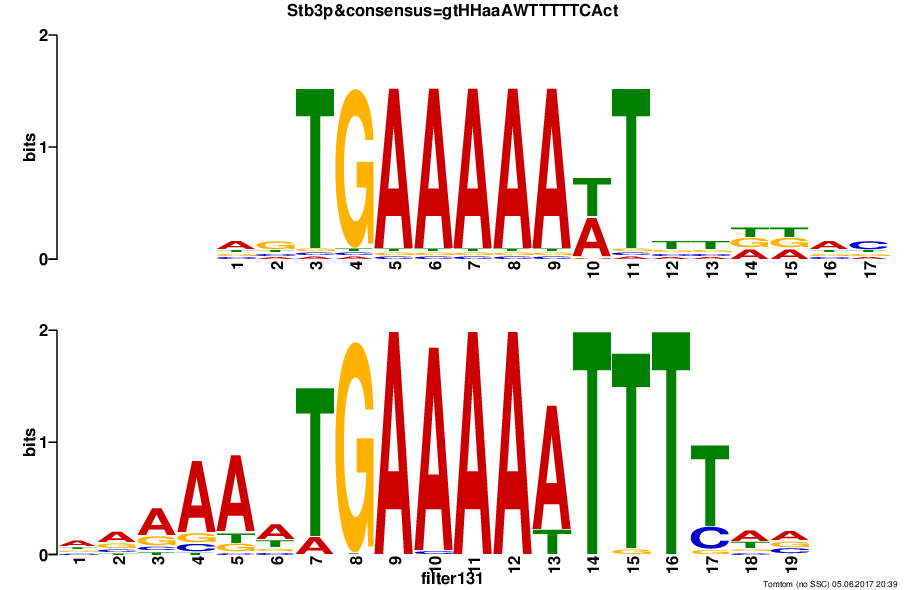
\includegraphics[width=\textwidth]{fig/tomtom/stb3p.png}
            \caption{STB3P}
    \end{subfigure}
    }
    \caption{(a) Predicted vs grounth truth (b-e) examples of recovered motifs}\label{fig:1}
\end{figure}

\subsection{Recovering Master Regulators}
A few studies have shown that yeast master regulators often manifest as key feature in prediction models \cite{Kundaje:2006ho}. To understand whether our model reflect the tran-regulatory component, we decided to rank the relative importance of the regulator module inputs, and test if such rank captures the master regulators in \textit{S. cerevisiae}. We reasoned that perturbations in regulators with high feature importance would lead to large change in the output. Therefore, we estimated the relative importance as the gradient (w.r.t to output) times the magnitude of input (G-by-I). We summed the G-by-I values across all genes and conditions to obtain the global estimate of feature importance. Notably, several master regulators such as USV1, YVH1, MSN4 appear as top features. 


\begin{table}[!hbt]
\caption{Rank of regulator module inputs}
\centering
 \begin{tabular}{|c | c|} 
 \hline
 Rank & Regulator \\
 \hline
 1 &  USV1 / YPL230W \\ 
 \hline
 2 & DAL80 / YKR034W \\
 \hline
 3 & XBP1 / YIL101C \\
 \hline
 4 & PPT1 / YGR123C \\
 \hline
 5 & LSG1 / YGL099W \\
 \hline
 6 & CIN5 / YOR028C \\
 \hline
 7 & YVH1 / YIR026C \\
 \hline
 8 & TPK1 / YJL164C \\
 \hline
 9 & GAC1 / YOR178C \\
 \hline
 10 & MSN4 / YKL062W \\
 \hline
\end{tabular}
\label{table:rank of regulator module inputs}
\end{table}

\subsection{\textit{in silico} Mutagenesis Reflects \textit{in vivo} Measurements}
Ultimately, the model should make predictions similar to actual experimental measurement, even for previously unseen conditions. Therefore, we performed \textit{in silico} knockout experiment on MSN2/4, where we replaced all instances of 'AGGGG' with neutral 'NNNNN', and reduced the expression level of MSN2/4 by 32 fold. MSN2/4 are activated under heat shock but are inactive under steady-state growth \cite{Sadeh:2011eg}. As expected, we observed that MSN2/4 target genes experience greater change under heat shock conditions than steady-state growth condition \ref{fig:target gene expression change}. We also compared our prediction against microarray measurement in a actual MSN2/4 knockout strain, and observed general agreement between the two (spearman correlation = 0.486, \ref{fig:predicted vs ground truth msn24 ko})


\begin{figure}
\centering
\begin{subfigure}{.5\textwidth}
  \centering
  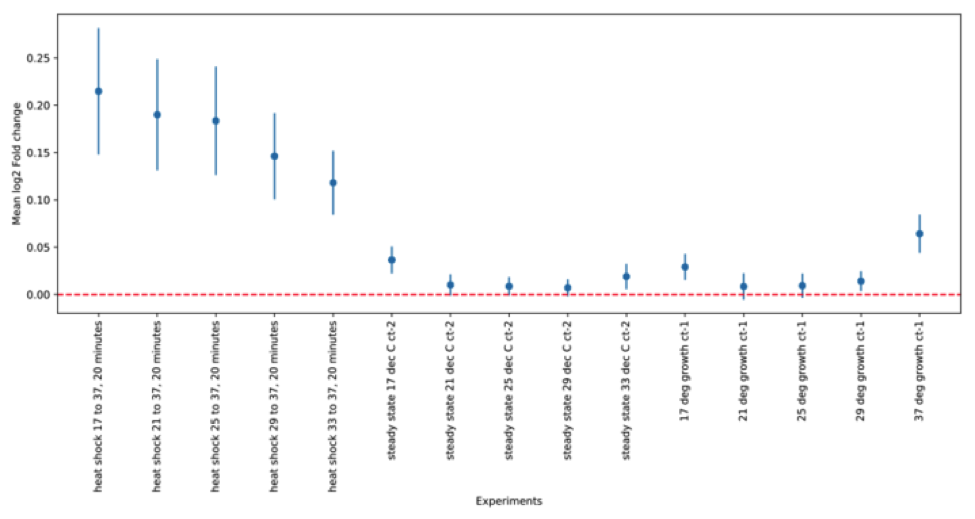
\includegraphics[width=1.0\textwidth]{fig/msn24_ko_target_genes.png}
  \caption{Target gene expression change}
  \label{fig:target gene expression change}
\end{subfigure}%
\begin{subfigure}{.5\textwidth}
  \centering
  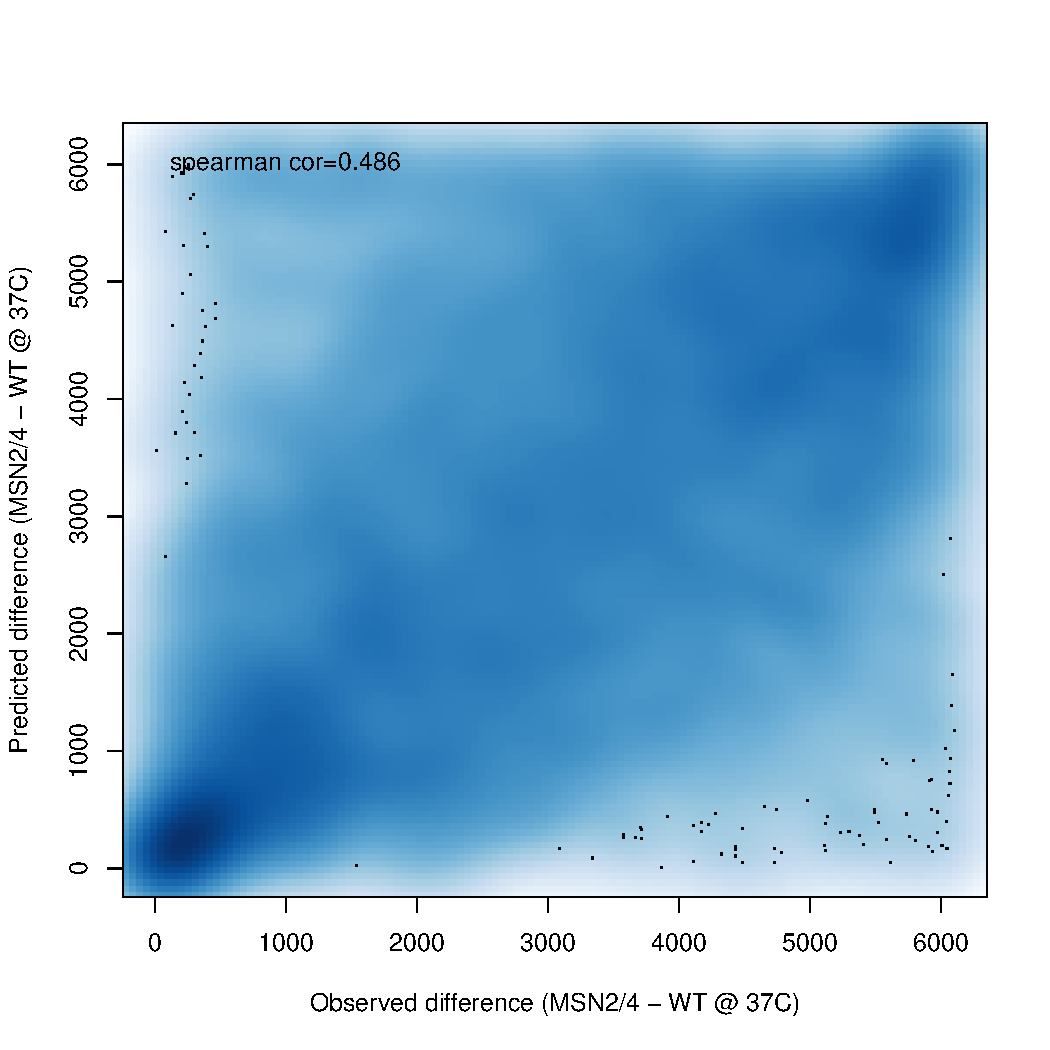
\includegraphics[width=1.0\textwidth]{fig/msn24_ko_37C_diff_expr_rank.pdf}
  \caption{Predicted vs ground truth}
  \label{fig:predicted vs ground truth msn24 ko}
\end{subfigure}
\caption{(a) The expression of MSN2/4 known target gene experience larger change under stress conditions. (b) Predicted expression change vs actual microarray experiment.}
\label{fig:fig2}
\end{figure}


% \section{Conclusion}
% We presented a deep learning architecture to model the genome-wide gene expression as the interaction between cis (1kb promoter sequence) and trans (signaling molecules and transcription factors). Our model performed the state-of-the-art model by ~17\%. It recovered known motifs, and attributed high feature importance to known master regulator. Through \textit{in silico} knockout experiments, our model make predictions similar to microarray measurements. 


\bibliographystyle{unsrt}
\bibliography{references}


\end{document}
